\section{Kamerakalibrierung}
%Um einen Punkt, welcher von der Kamera bzw. der Queue-Erkennung erfasst wurde, korrekt in das Spielfeld zu projezieren, müssen folgende Schritte durchlaufen werden:\\
%Der gegebene Punkt, welcher in einem 2D Vektor vorliegt, muss in das gegebene Spielfeldkorrdinatensystem transformiert werden. Hierfür muss das Spielfeld zunächst von der Kamera erkannt werden um anschließend im Kamerakoordinatensystem festgehalten zu werden. Da das Kamerabild eine natürliche Verzerrung des Bildes beinhaltet, muss ebenso diese Verzerrung entzerrt werden. Dies wird mit Hilfe eines bekannten Musters, welches in diesem Projekt ein Schachbrettmuster ist, bewerkstelligt, in welchem signifikante Eckpunkte erkannt, daraus die Verzerrung ermittelt und entzerrt werden. Nachdem dies erfolgt ist, kann ein erkannter und entzerrter Punkt aus der Kamera in das Spielfeldkoordinatensystem übertragen werden. Hierfür muss eine Umrechnung erfolgen, da das Kamerakoordinatensystem oben links den (0,0)-Punkt hat und das Spielfeld unten rechts.

%\subsection{Einleitung}
%Sobald die Anwendung gestartet wird, wird die Kamera verbunden und ein Timer fragt alle 16ms ab, ob die Kalibrierung gestartet werden soll. Wenn dem so ist, wird auf dem Spielfeldbereich ein Schachbrettmuster gerendert und nach jedem Ablauf des Timers, hier dem entsprechend alle 16ms, Fotos aufgenommen. Sobald eine festgelegte Grenze von aufgenommenen Fotos erreicht wurde, werden diese ausgewertet, ob das Schachbrettmuster auf diesen Fotos erkannt wurde. Falls dem nicht so ist, werden erneut Fotos aufgenommen. Ansonsten werden die Eckpunktkoordinaten des erkannten Musters gespeichert und damit die Entzerrung ausgeführt. Im Anschluss kann ein, von der Queue-Erkennung erfasster Punkt, entzerrt und ins Spielfeld übertragen werden.

\subsection{Darstellung des Erkennungsmusters}
Um die Kamera kalibrieren und das Kamerabild entzerren zu können, muss die Kamera ein bekanntes Erkennungsmuster finden und in diesem bestimmte Eckpunkte erfassen und auswerten können. In unserem Projekt wird ein Schachbrettmuster genutzt, von welchem die inneren Eckpunkte erkannt werden. Hierfür muss die Anzahl der Kacheln in der Horizontalen = $Hor$, sowie in der Vertikalen = $Vert$, bekannt bzw. festgelegt sein, um für jede Kachel die selbe Höhe und Breite zu haben und trotzdem die gesamte Höhe und Breite des Spielfeldes abzudecken. Die Höhe und Breite wird wie folgt berechnet:\\
$Hoehe_{Kachel} = \frac{Hoehe_{Game}}{Vert}$, $Breite_{Kachel} = \frac{Breite_{Game}}{Hor}$\\
Nun wird für jedes $i \in [1,Hor]$ alle $j \in [1,Vert]$ eine Kachel gerendert mit den Koordinaten oben links ($i \cdot Hoehe_{Kachel}$, $j \cdot Breite_{Kachel}$) und den Koordinaten unten rechts ($(i+1) \cdot Hoehe_{Kachel}$, $(j+1) \cdot Breite_{Kachel}$). Zudem wird bei jeder neuen Kachel in der Horizontalen die invertierte Farbe der vorherigen Kachel als Grundfarbe gewählt und in der Vertikalen für die erste Kachel die invertiere Farbe der darüber liegenden Kachel gewählt, damit das klassische Schwarz-Weiß-Muster eines Schachbretts visualisiert wird.
\begin{figure}[h]
	\label{fig:chessboard}
	\centering
	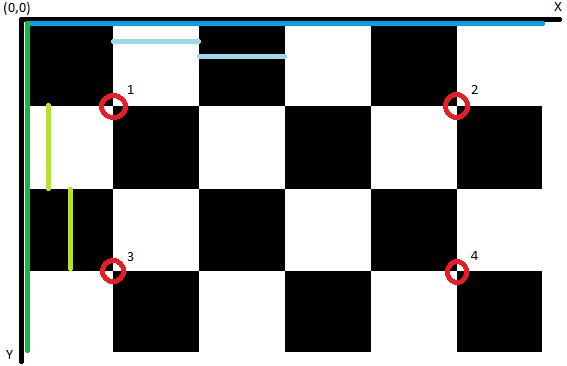
\includegraphics[scale=0.8]{bilder/schachbrett.png}
	\caption{Schachbrettmuster rendern}
\end{figure}

\subsection{Entzerrung des Kamerabildes/Punktes}
%Bildkoordinaten = BK, Weltkoordinaten = WK, Patterneckpunkte = PE, Vector 2/3 Point = 2/3V\\
%Nimmt 20 Fotos auf und wertet diese dann in der $Calibration$ aus:\\
%$patternWorldCoordinates$ = 3V mit $(x*a,y*a,0)$ für alle $x \in Hor-1$ für alle $y \in Vert-1$ und $a$ = Kantenlänge für Kachel in WK\\
%$patternCorners$ = 2V Speicher für PE in BK\\
%$patternWorldBuffer$ = 3V Speicher für PE in WK\\
%$pointBuffer$ = 2V Zwischenspeicher für PE in BK (wird für jedes Bild neu initialisiert)\\

\subsection{Punktübertragung von Kamera in Spiel}
Der letzte Abschnitt der Kamerakalibierung stellt das Übertragen eines von der Queue-Erkennung gegebenen Punktes, welcher sich im Kamerakoordinatensystem befindet, in das Spielfeldkoordinatensystem um diesen dann in den Spielmechanismus als Queueposition einzubinden.
Um dies einwandfrei zu ermöglichen, müssen die äußersten Eckpunkte des, von der Kamera erfassten, Schachbrettmusters im Kamerakoordinatensystem bekannt sein. Da allerdings nur die Eckpunkte auf der Innenseite des äußersten Ringes des Schachbretts erkannt werden, müssen die ganz äußersten Eckpunkte wie folgt berechnet werden:\\
$Lila_{min} = Gruen_{min} - Rot_{min}$\\
$Lila_{max} = Rot_{max} - Gruen_{max}$
\begin{figure}[h]
	\label{fig:chessboard}
	\centering
	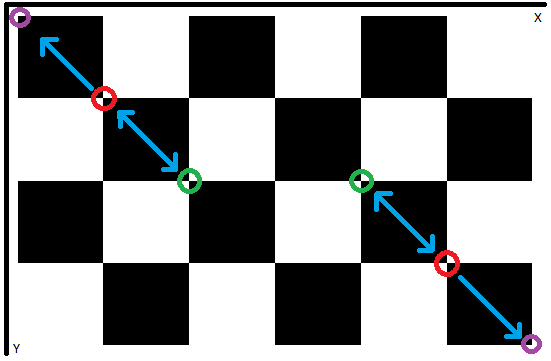
\includegraphics[scale=0.8]{bilder/schachbrettdiff.png}
	\caption{Schachbrettmuster Eckpunkte}
\end{figure}\\
Nun sind die äußersten Eckpunkte des Spielfeldes im Kamerakoordinatensystem bekannt und es ist möglich einen beliebigen 2D Punkt in das Spiel zu projezieren. Hier wird unter zwei Fällen unterschieden. Entweder liegt der übergebene Punkt der Kamera im Spielbereich oder nicht: $X \in [x_{min}, x_{max}]$ und $Y \in [y_{min},y_{max}]$.
Sofern dieser Punkt im Spielbereich liegt, wird dieser Punkt $P$ in das Spielkoordinatensystem projeziert, was wie folgt berechnet wird:\\
$X = \dfrac{(P.x - MIN.x) * UR}{(MAX.x - MIN.x)}$, 
$Y = \dfrac{(MAX.y - P.y) * OL}{(MAX.y - MIN.y)}$
\begin{figure}[h]
	\label{fig:chessboard}
	\centering
	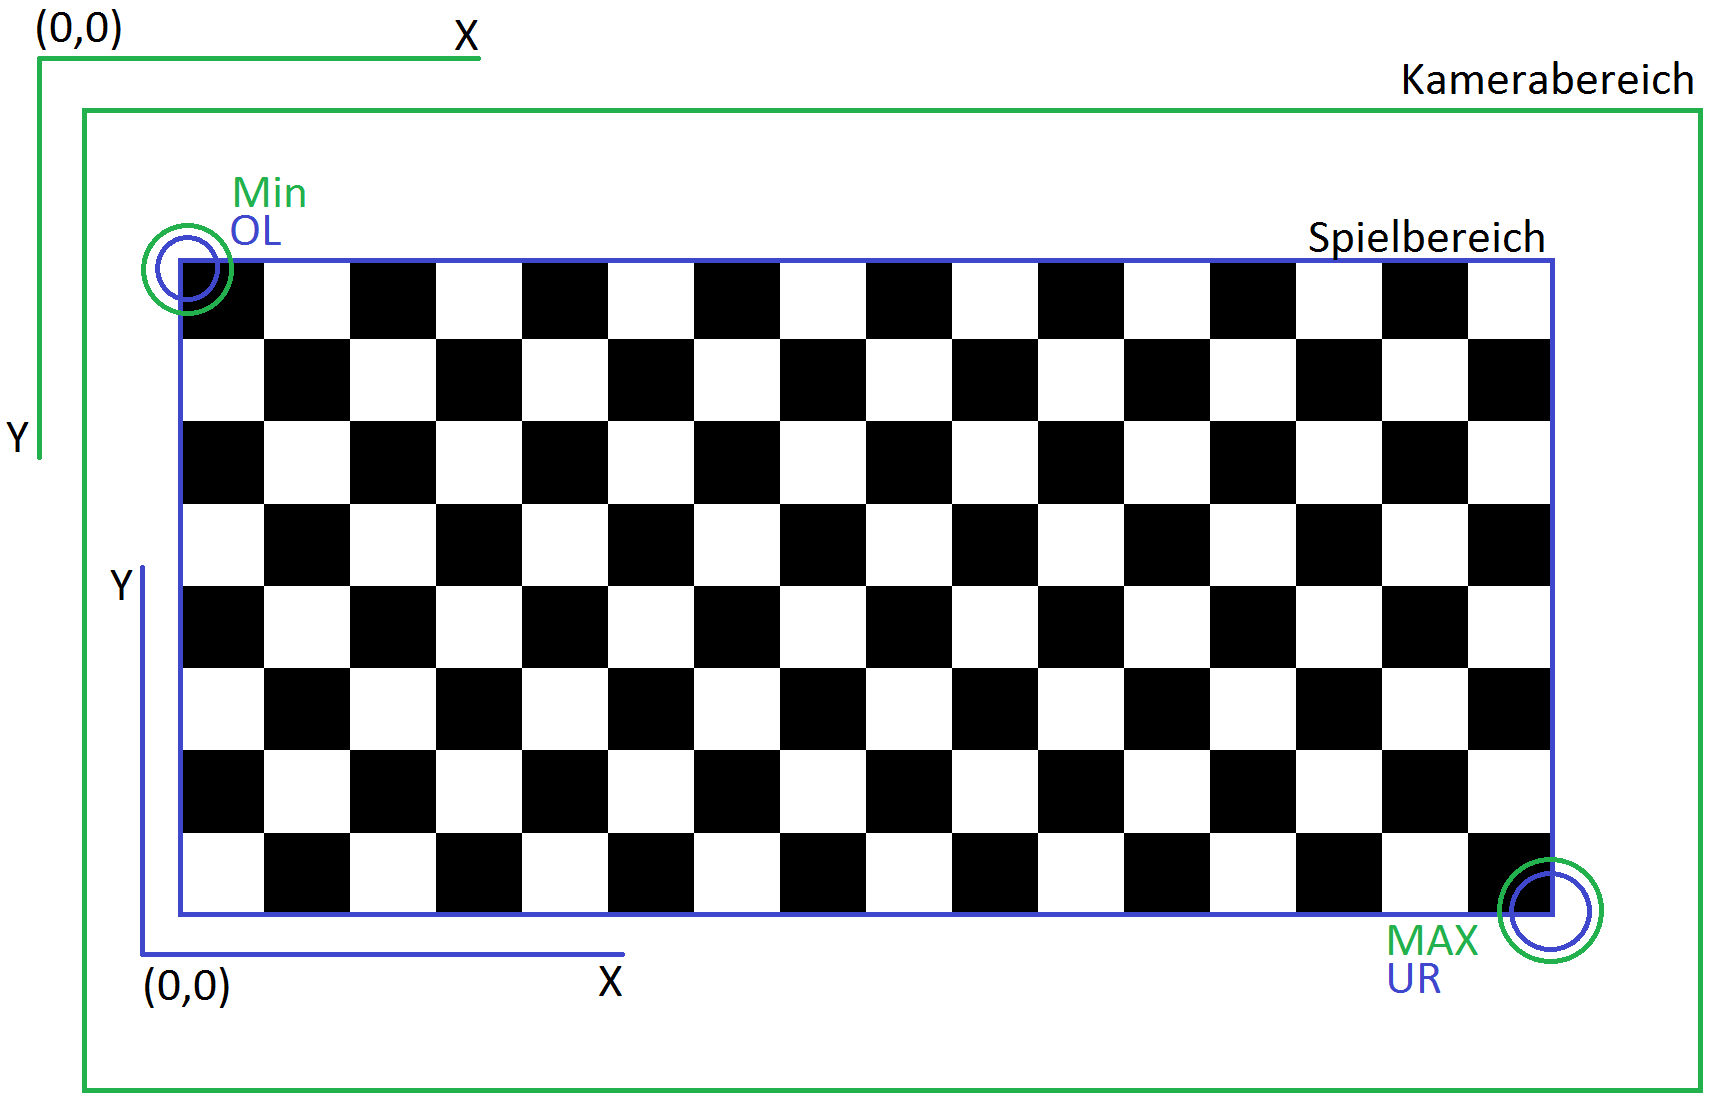
\includegraphics[scale=0.3]{bilder/schachbrettkamera.png}
	\caption{Kamera- und Spielkoordinatensystem}
\end{figure}\\
